\documentclass{article}
\usepackage[portrait, margin=1in]{geometry}
\usepackage{graphicx} 
\graphicspath{{/Users/danpost/mystery_ca_gas_surcharge/output/ca_city_rack_analyses}}
\usepackage{amsmath}
\usepackage{hyperref}
\usepackage{booktabs}
\usepackage{array}

\begin{document}

\title{Analysis of Rack Prices in California} 

\maketitle

\section{Summary}
This memo attempts to summarize the chain of prices in CA's gasoline market and contextualize these price patterns with respect to the California Mystery Gas Surcharge (MGS). The central takeaways are:
\begin{itemize} 
	\item The spot price differential between CA and the rest of the country went through a temporary spike following the Torrance Refinery Fire in February, 2015; however, that spot price differential quickly came down to pre-Torrance levels while the MGS remained elevated. 
	\item A persistent increase in the difference between rack prices throughout California and the Los Angeles spot price, in real terms, coincided with the MGS. It appears that the MGS is being generated in between the spot and rack markets. 
	\item There has been no apparent change in the pattern of the difference between rack and retail prices throughout California following the Torrance fire.
	\item Specific patterns with respect to rack prices vary city-to-city, but overall the gap between unbranded and branded gasoline prices have widened in the years since the Torrance fire. 
	\item Overall, variance across rack prices has significantly increased post-Torrance fire.
	\item In particular, Shell-branded, Chevron-branded, and ConocoPhillips-branded gasoline have lead the way in outpacing overall rack prices significantly in a pattern dating to around the Torrance fire. 
	\item On the other hand, Valero-branded gasoline has, across the board, lagged behind overall rack prices since the Torrance fire.
\end{itemize} 

\section{Tracing Chain of Prices}

Generally, there are 4 `stages' of prices that we can trace out in gasoline markets: 
\begin{enumerate} 
	\item NYMEX Gasoline Futures
	\begin{itemize}
		\item National-level
	\end{itemize}
	\item Spot Prices 
	\begin{itemize}
		\item Spot Market-level: California has 2 spot markets: Los Angeles and San Francisco
		\item Spot prices don't have to publicly reported, so data on San Francisco, the less significant spot market of the two, is sparse and not as reliable. Thus, for this analysis, I focus on Los Angeles spot prices
	\end{itemize}
	\item Rack prices 
	\begin{itemize}
		\item These are located at distribution points between retail gasoline stations and spot markets. There are 12 rack fuel locations in CA, with varying degrees of importance
	\end{itemize}
	\item Retail gasoline prices
	\begin{itemize}
		\item These vary gas-station-to-gas-station and are `composed' of all prices from earlier in the supply chain
	\end{itemize}
\end{enumerate}

\subsection{Spot-Gasoline Futures Differential}
First, we can compare Los Angeles spot prices to the rest of the country, by analyzing the difference between the Los Angeles and NY Harbor/US Gulf Coast spot prices (I take the average of the NY Harbor and Gulf Coast Spot Prices). 

\centering 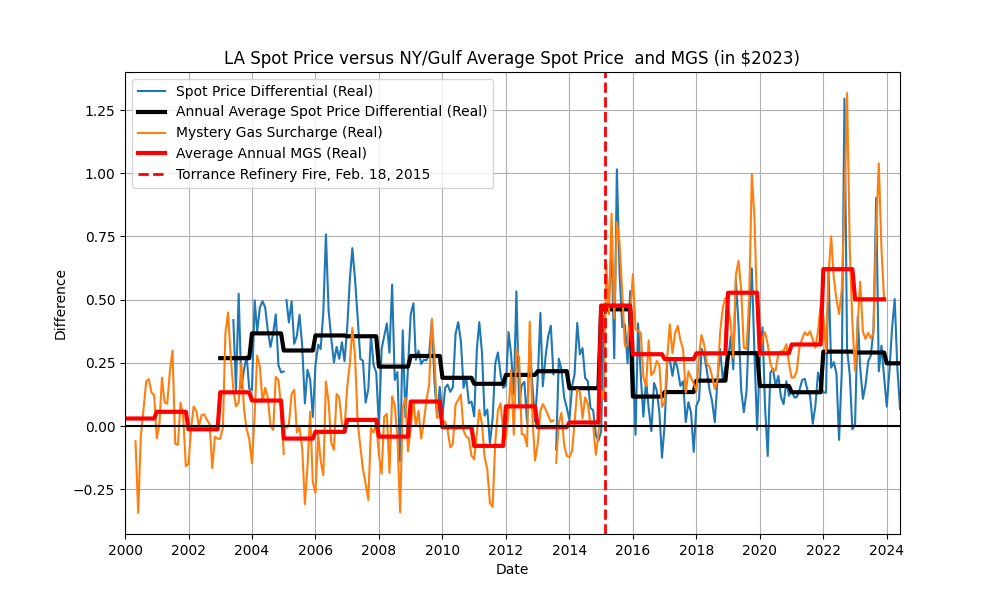
\includegraphics[width=5.5in]{spot_differential.png} \\
\raggedright LA Spot Prices are consistently higher than the rest of the country. This makes sense: most refiners and drillers are located in the Gulf Coast and there is a pipeline connecting the Gulf Coast to Linden, NJ (near NY Harbor, the Colonial Pipeline). On the other hand, the only way for gas to make its way to California from the Gulf Coast is on ships that are subject to the Jones Act, significantly raising costs in the absence of a direct pipeline connection. 

Also, the spot price differential has little to do with the MGS; the MGS spiked when the spot difference did, due to a short-term fluctuation in supply associated with the Torrance Refinery Fire. However, the spot price came down and pre-Torrance levels while the MGS remained elevated and persistent, even increasing.

\subsection{Rack-Spot Differential}
The next step in the distributional chain are rack prices. These are the prices that distributors charge at `rack fuel locations', where gasoline purchased at the spot market--either San Fransisco or Los Angeles--is transported before being further transported to gasoline stations. Whereas spot prices are publicly available for free, rack prices are not.\footnote{Rack price data was taken from the Bloomberg Terminal.} \\
\centering 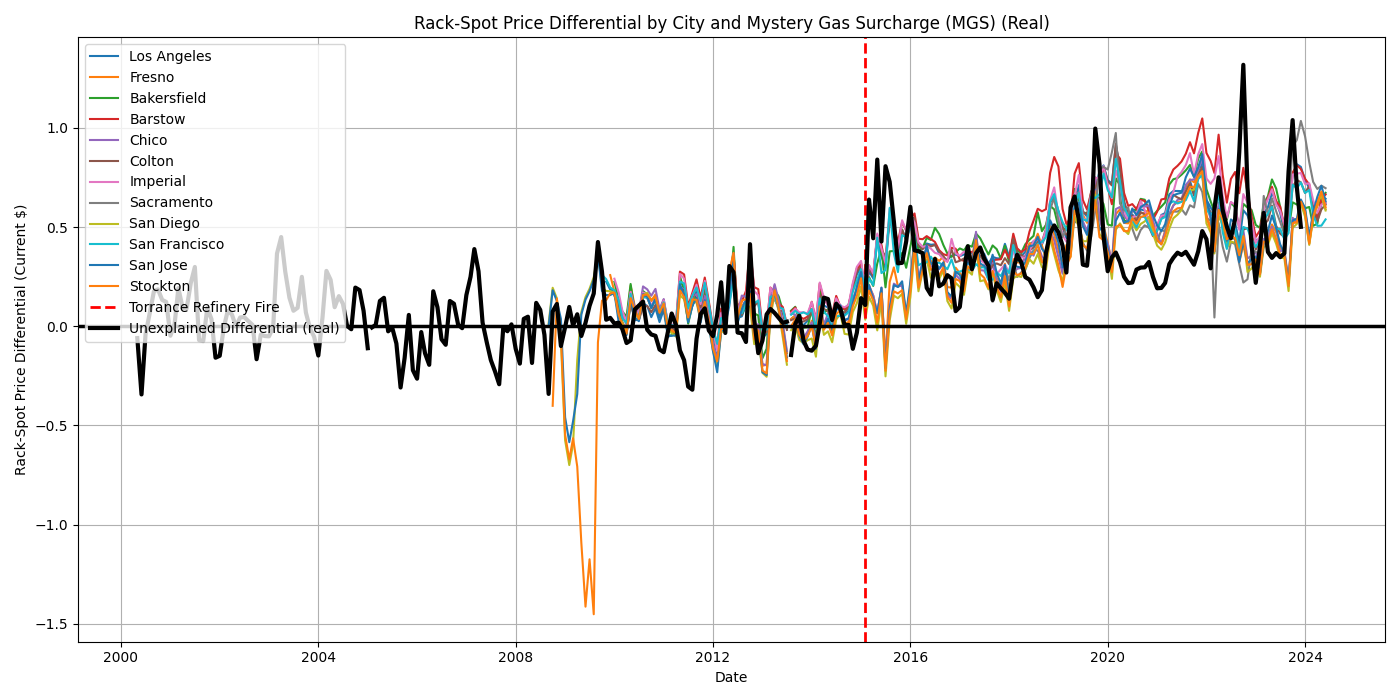
\includegraphics[width=5.5in]{rack_spot_differentials.png}

\raggedright There's a high degree of correlation here, as the rack price spreads for each city spiked at nearly the same time as Torrance Refinery Fire and have remained elevated ever since. This would suggest that it's \textit{not} downstream but upstream where the MGS is being generated post-2015. 

\subsection{Retail-Rack Differential}
The next step is to compare rack with retail prices over time.\footnote{The retail price used is the \textit{overall} CA average retail price.} \\
\centering 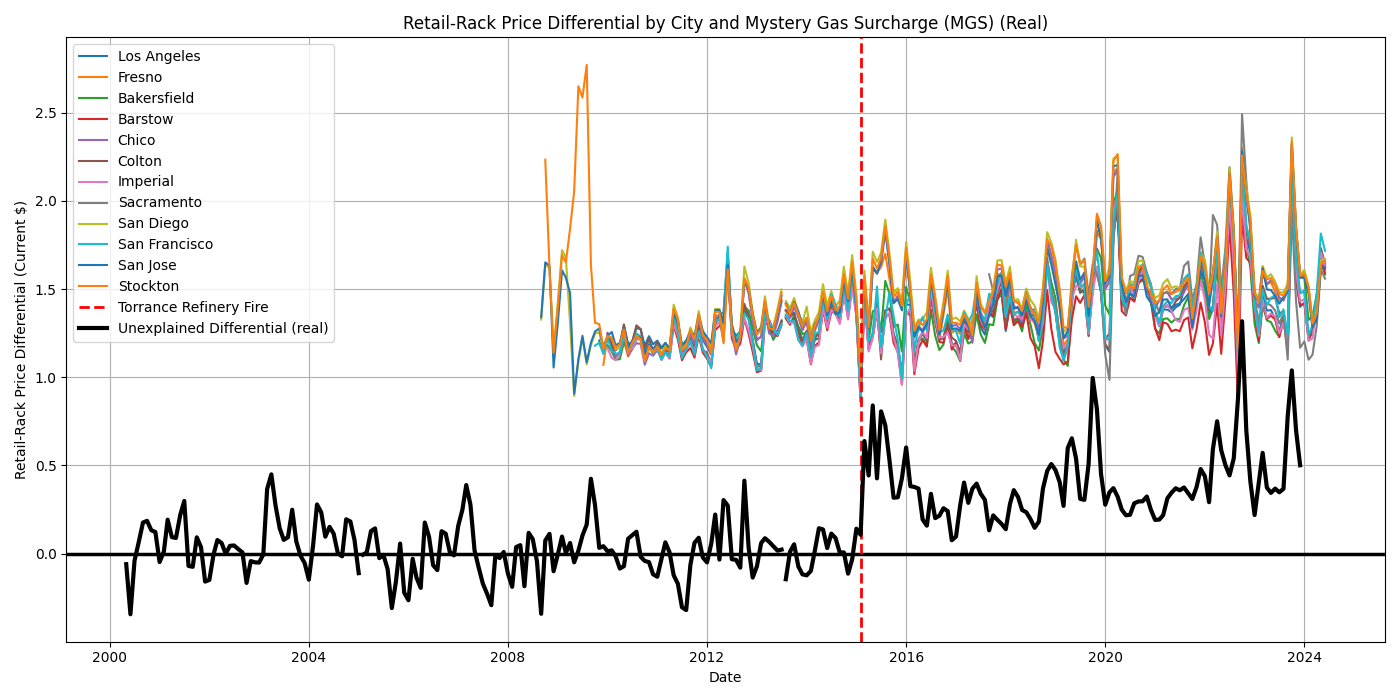
\includegraphics[width=5.5in]{retail_rack_differentials.png} \\
\raggedright Retail prices have remained elevated above rack prices at a fairly consistent margin, and the pattern in this differential did not seem to change after the Torrance Refinery Fire.

\section{Detailed City-by-City Analysis of Rack Prices}
Bloomberg provides very granular data on rack prices by rack fuel location, with different prices by: 1) refiner, 2) whether gasoline is branded/unbranded, 3) location of refiner (these are usually cities very close to the rack fuel location itself if not the city itself), and 4) which company is distributing the gasoline after it is refined.\footnote{Note that these are rack prices corresponding to CARB, 87 RFG, blended with 10\% Ethanol. This is in accordance to my and Severin Borenstein's methodology, which assumed maximum pass-through costs for the Low Carbon Fuel Standard (LCFS) program. This assumed that all gasoline sold was E-10, the most common blend of gasoline in the US, and of the lowest quality (hence I selected 87 RFG rather than 89 RFG and 91 RFG which also have corresponding rack fuel prices in the Bloomberg Terminal).} Below I have plotted the real rack price spreads for each of these granular variables: this is calculated as the ((granular rack price) - (overall rack price index))/(price deflator). \\
The rack fuel locations included in this analysis are: 
\begin{itemize} 
	\item Los Angeles (pop. 3,822,000)
	\item San Diego (pop. 1,381,000
	\item San Jose (pop.971,233)
	\item San Francisco (pop. 808,437)
	\item Fresno (pop. 545,567)
	\item Sacramento (pop. 528,001)
	\item Bakersfield (pop. 410,647)
	\item Stockton (pop. 321,819)
	\item Chico (pop. 101,299)
	\item Colton (pop. 53,918)
	\item Barstow (pop. 25,231)
	\item Imperial (pop. 21,233)
\end{itemize}

\subsection{Location of Refineries in California with Production}
For context, here is a list of refiners in CA.\footnote{Note that I have only included refineries that are currently producing CARB gasoline. \href{https://www.energy.ca.gov/data-reports/energy-almanac/californias-petroleum-market/californias-oil-refineries}{Source}. } 
\begin{tabular}{|>{\raggedright}p{4cm}|>{\centering}p{3cm}|>{\centering}p{3cm}|>{\centering}p{3cm}|>{\centering\arraybackslash}p{2cm}|}
\hline
\textbf{Refinery Name} & \textbf{Associated Rack Location} & \textbf{Barrels Per Day} & \textbf{\% of California Crude Oil Capacity} & \textbf{CARB Gasoline} \\
\hline
Marathon Petroleum Corp., Los Angeles Refinery & Los Angeles & 363,000 & 21.22\% & Yes \\
\hline
Chevron U.S.A. Inc., El Segundo Refinery & Los Angeles & 269,000 & 15.73\% & Yes \\
\hline
Chevron U.S.A. Inc., Richmond Refinery & San Francisco & 245,271 & 14.34\% & Yes \\
\hline
PBF Energy, Torrance Refinery & Los Angeles & 160,000 & 9.35\% & Yes \\
\hline
PBF Energy, Martinez Refinery & San Francisco & 156,400 & 9.14\% & Yes \\
\hline
Valero Energy, Benicia Refinery & San Francisco & 145,000 & 8.48\% & Yes \\
\hline
Phillips 66, Los Angeles Refinery & Los Angeles & 139,000 & 8.13\% & Yes \\
\hline
Phillips 66, Rodeo San Francisco Refinery & San Francisco & 90,200 & 5.27\% & Yes \\
\hline
Valero Energy, Wilmington Refinery & Los Angeles & 85,000 & 4.97\% & Yes \\
\hline
Kern Energy, Bakersfield Refinery & Bakersfield & 26,000 & 1.52\% & Yes \\
\hline
San Joaquin Refining Company Inc., Bakersfield Refinery & Bakersfield & 15,000 & 0.88\% & No \\
\hline
\end{tabular}

\subsection{Los Angeles}
\centering 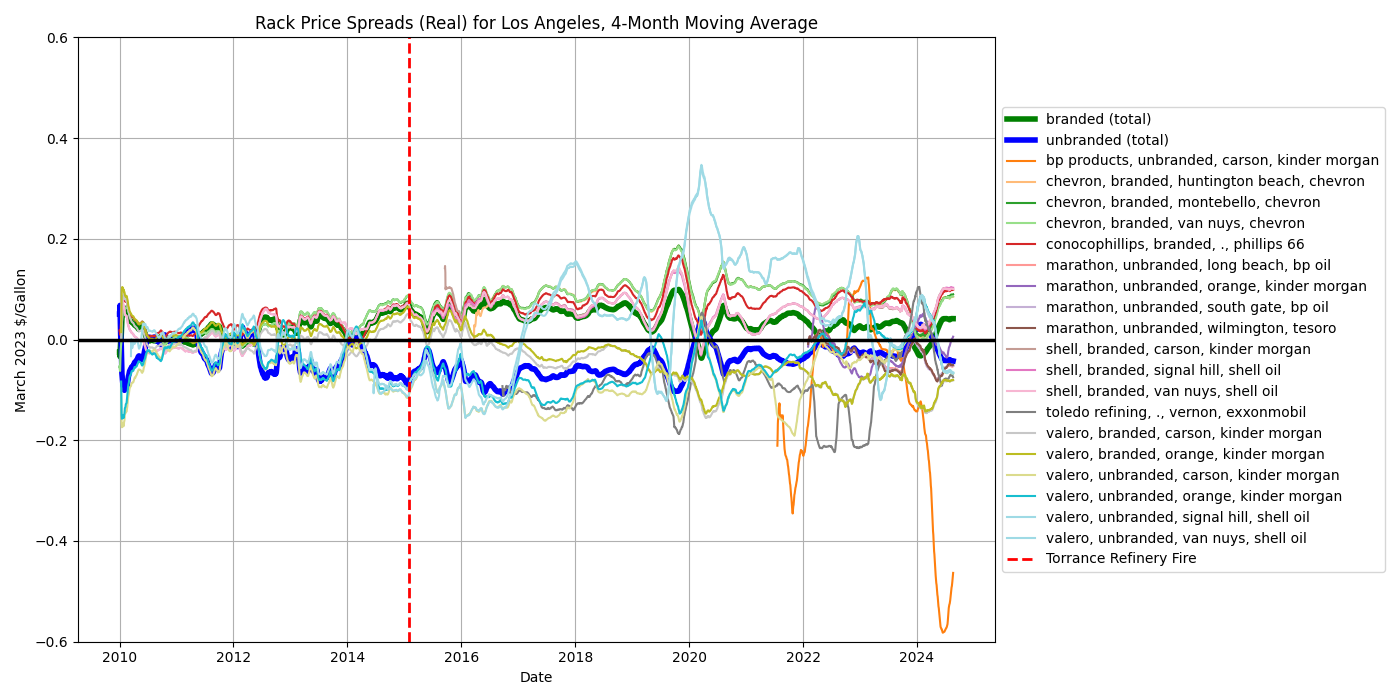
\includegraphics[width=5.5in]{los angeles_spread.png}\\
\raggedright In Los Angeles, the branded-unbranded differential is closing. Chevron-branded, ConocoPhillips-branded, and Shell-branded (in each case the refiner being the same as the distributor) appear the most elevated.

\subsection{San Diego}
\centering 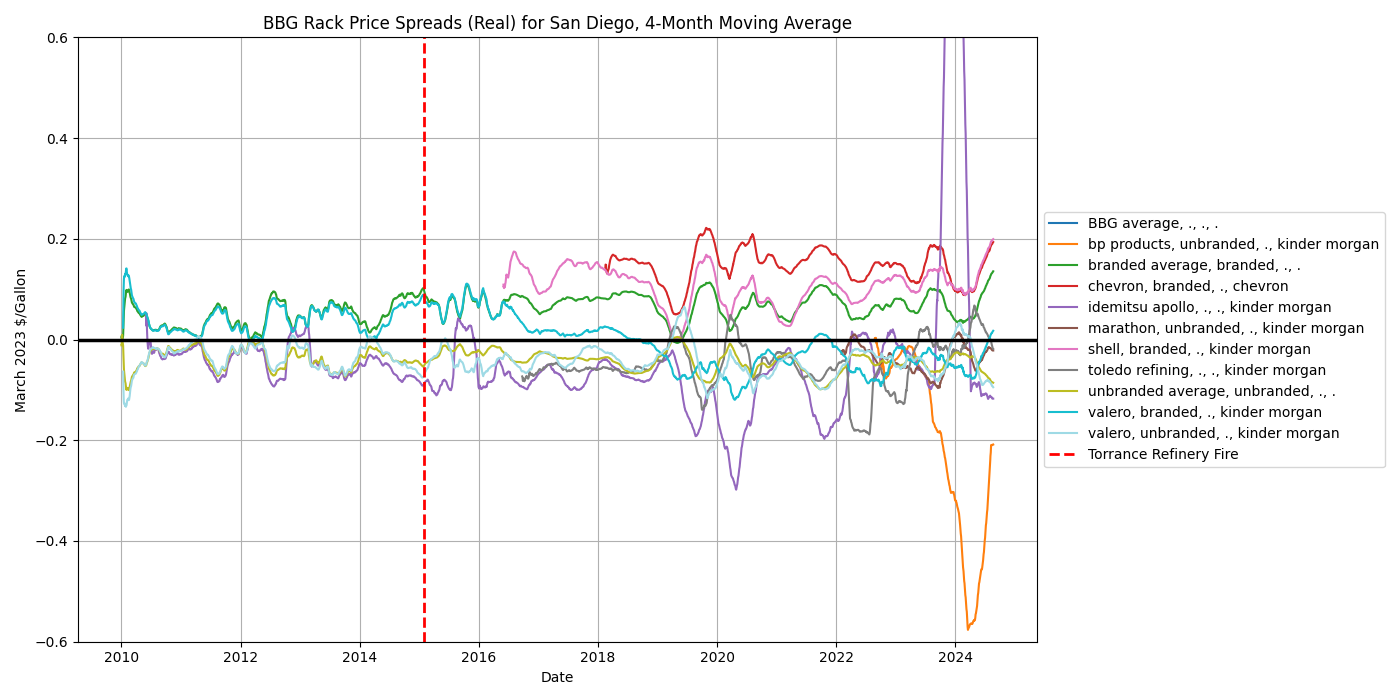
\includegraphics[width=5.5in]{san diego_spread.png}\\
\raggedright In San Diego, the branded-unbranded difference has persisted; here, Chevron-branded and Shell-branded (in each case the refiner being the same as the distributor) appear the most elevated. 

\subsection{San Jose}
\centering 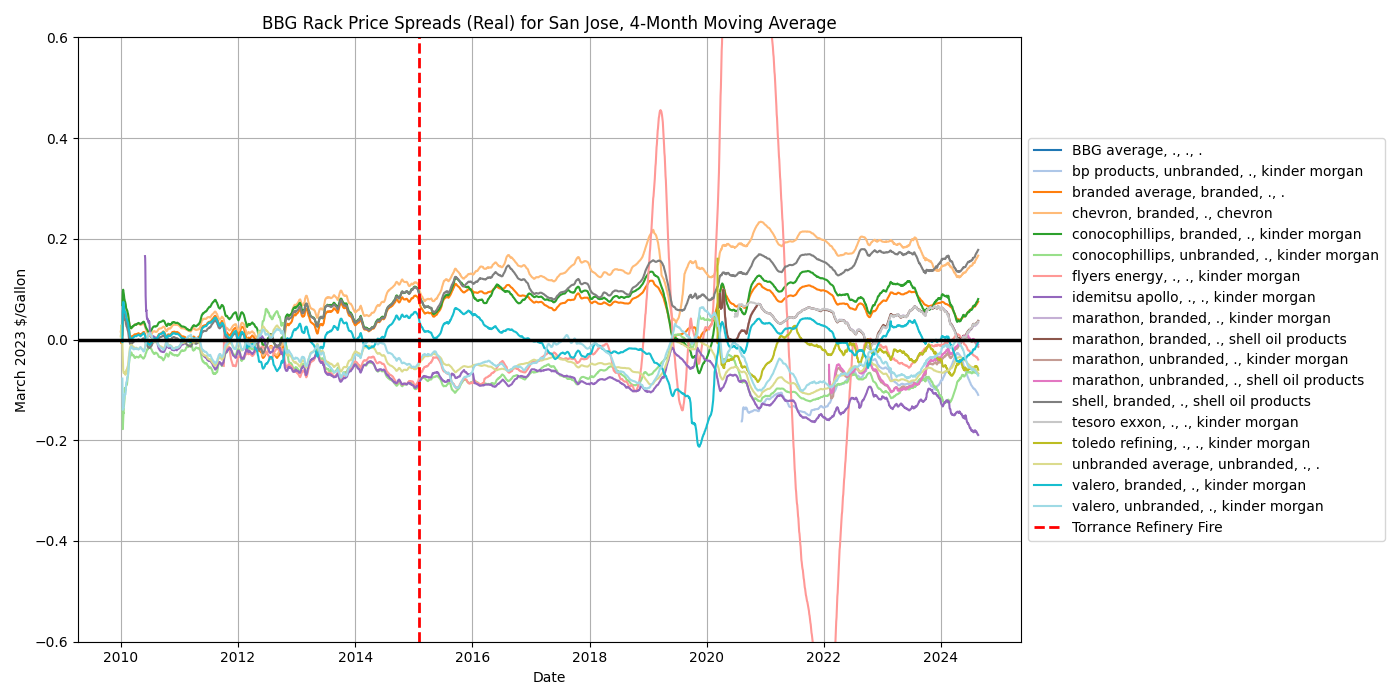
\includegraphics[width=5.5in]{san jose_spread.png}\\
\raggedright San Jose has a similar pattern for the branded-unbranded price difference. Here, it appears that Chevron-branded, Shell-branded, and ConocoPhillips-branded gasoline are the most elevated (each distributed by the refiner, except for ConocoPhillips, which is distributed by Kinder Morgan). 

\subsection{San Francisco}
\centering 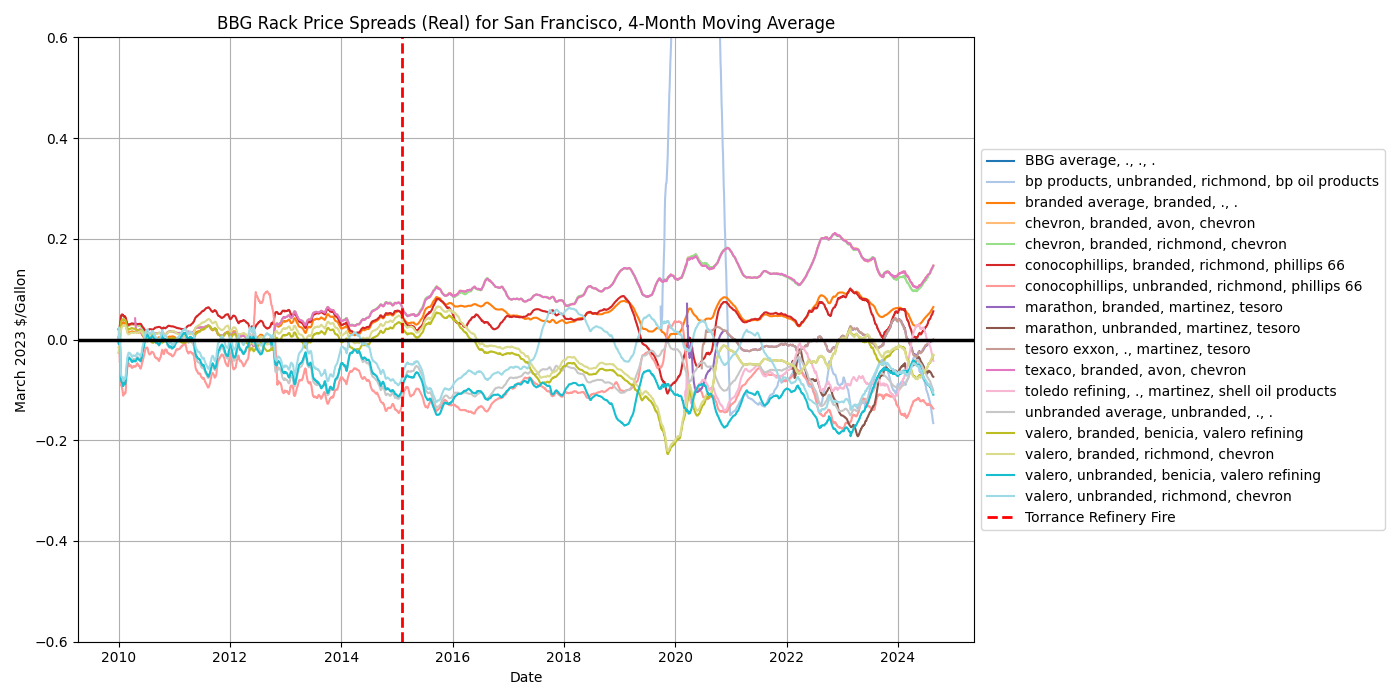
\includegraphics[width=5.5in]{san francisco_spread.png}\\
\raggedright SF has a similar branded-unbranded differential as the cities shown above. Over time, the Chevron-branded and Shell-branded (in both cases the refiner is also the distributor) appear to be the most elevated and growing spreads.

\subsection{Fresno}
\centering 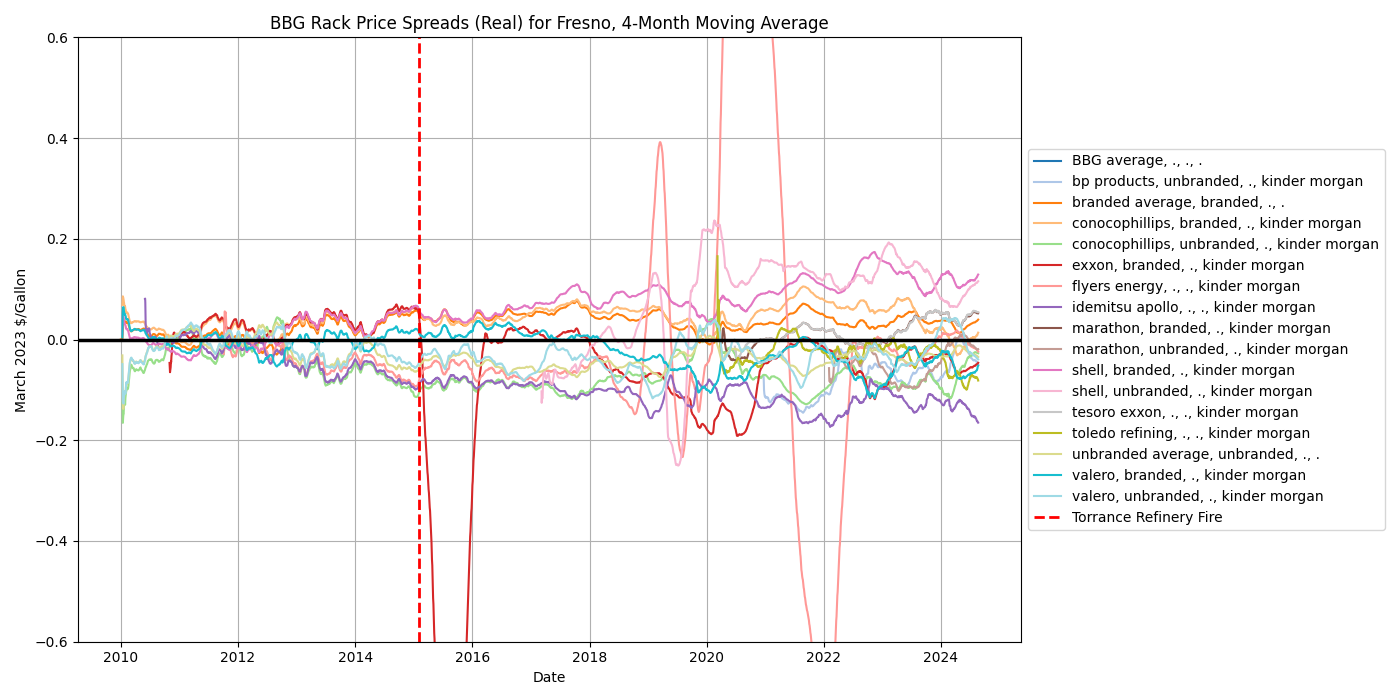
\includegraphics[width=5.5in]{fresno_spread.png}\\
\raggedright The branded-unbranded difference is lesser for Fresno than most cities. Here Shell-branded and Shell-unbranded, and Tesoro Exxon are all elevated (all three being distributed by Kinder Morgan).\footnote{I suspect that the Shell-unbranded is distorting the branded-unbranded difference by pulling the unbranded average upwards; this is the only rack fuel location where there is a variable corresponding to shell unbranded gasoline.}

\subsection{Sacramento} 
\centering 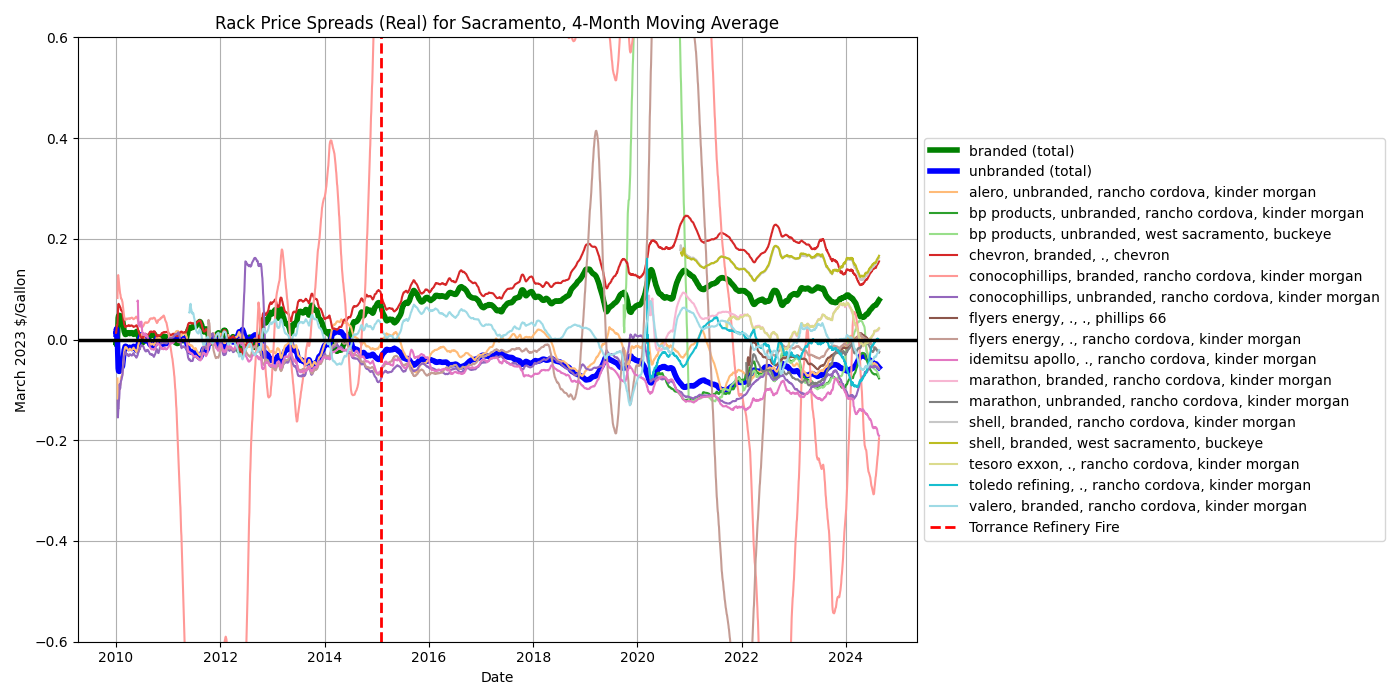
\includegraphics[width=5.5in]{sacramento_spread.png}\\
\raggedright Sacramento has very volatile price spreads over time. However, it's very clear that the branded-unbranded difference opened up around 2015 and has persisted. Chevron-branded and Shell-branded gasoline are the most elevated; for Sacramento, only this Chevron-branded gasoline is also distributed by Chevron, while the shell is distributed by Buckeye.

\subsection{Bakersfield}
\centering 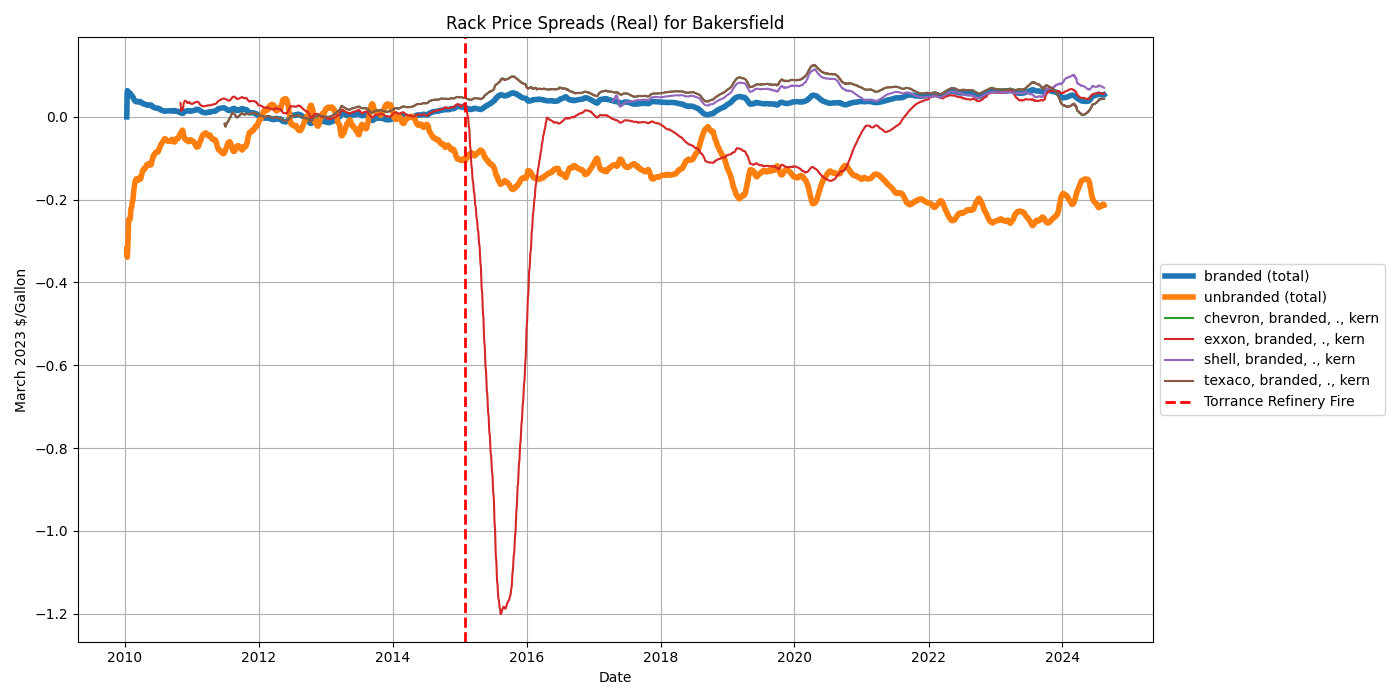
\includegraphics[width=5.5in]{bakersfield_spread.png} \\
\raggedright Bakersfield is relatively sparse. All branded gasoline is distributed by Kern and appear to be at approximately the same level, although Exxon has historically been volatile.

\subsection{Stockton}
\centering 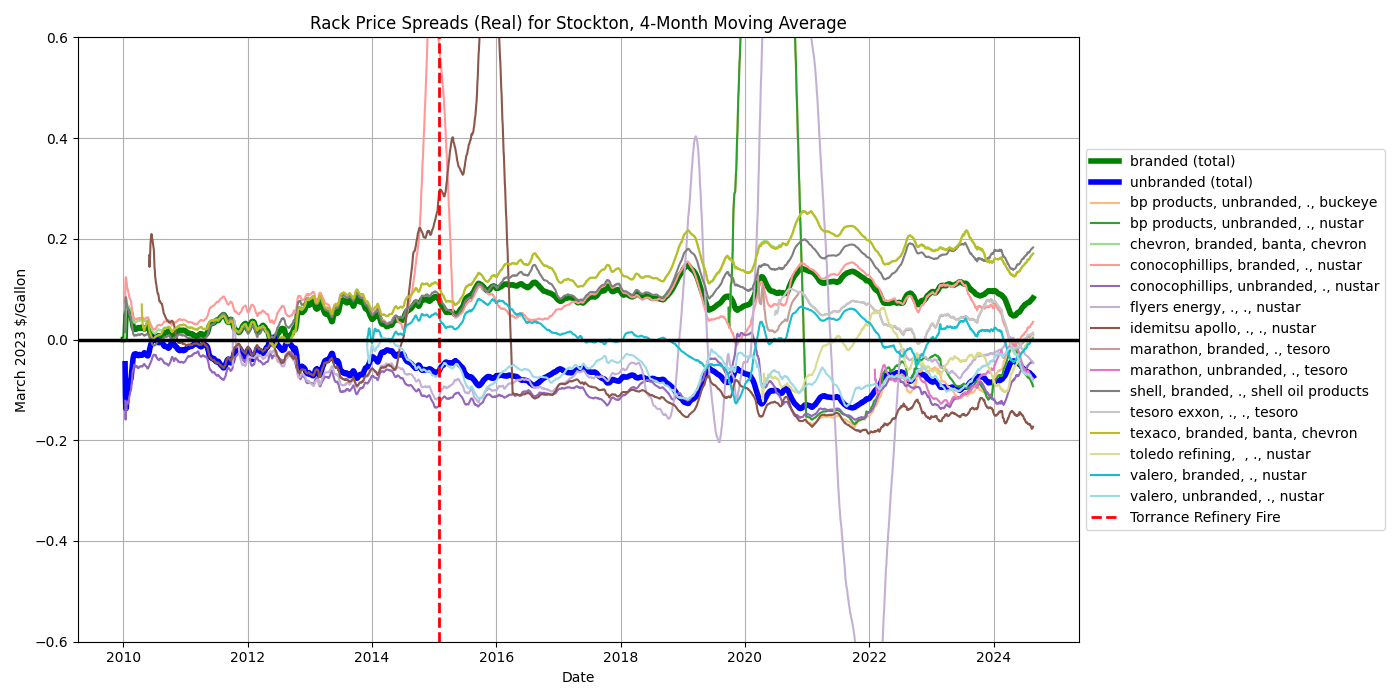
\includegraphics[width=5.5in]{stockton_spread.png}\\
\raggedright Stockton exhibits the usual branded-unbranded spread. Here, Texaco-branded and Shell-branded are the most elevated rack prices (the former is distributed by Chevron and the latter is distributed by Shell). 

\subsection{Chico}
\centering 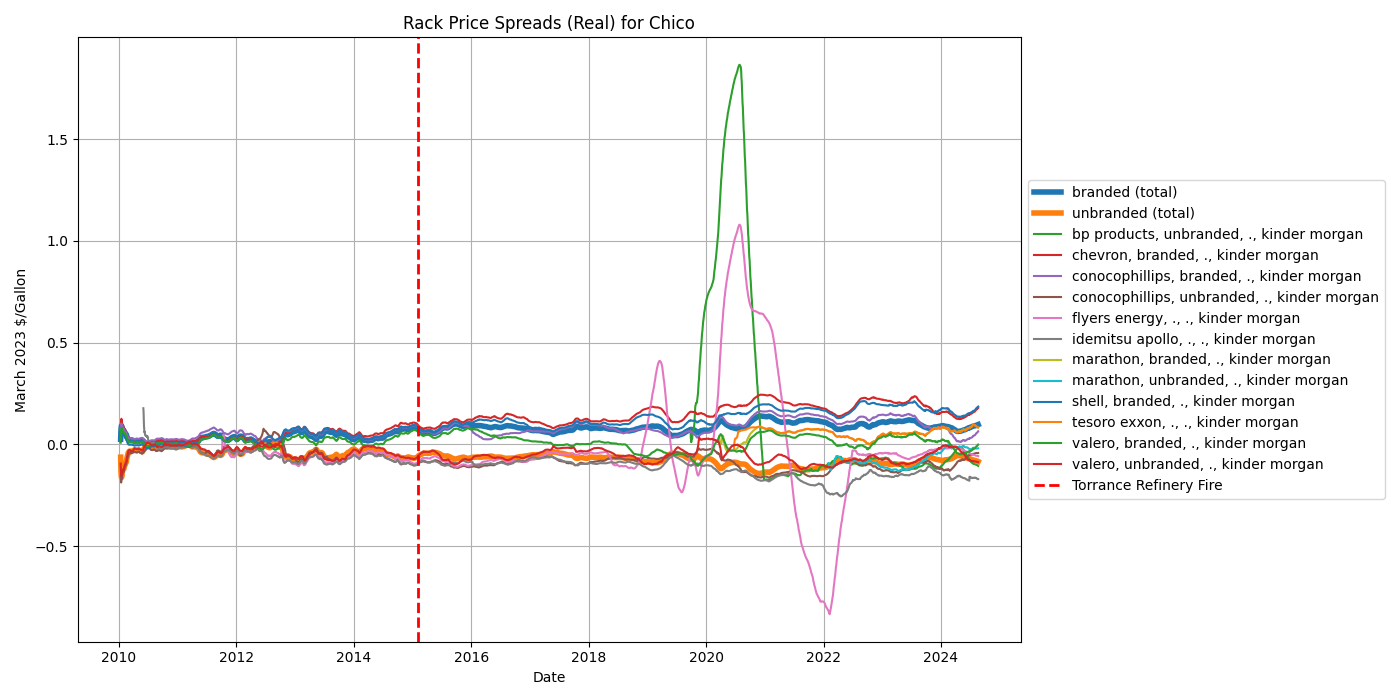
\includegraphics[width=5.5in]{chico_spread.png}\\
\raggedright Chico exhibits the usual branded-unbranded spread, and Chevron-branded, Shell-branded, and ConocoPhillips-branded gasoline are the most elevated. All gasoline is distributed by Kinder Morgan.

\subsection{Colton}
\centering 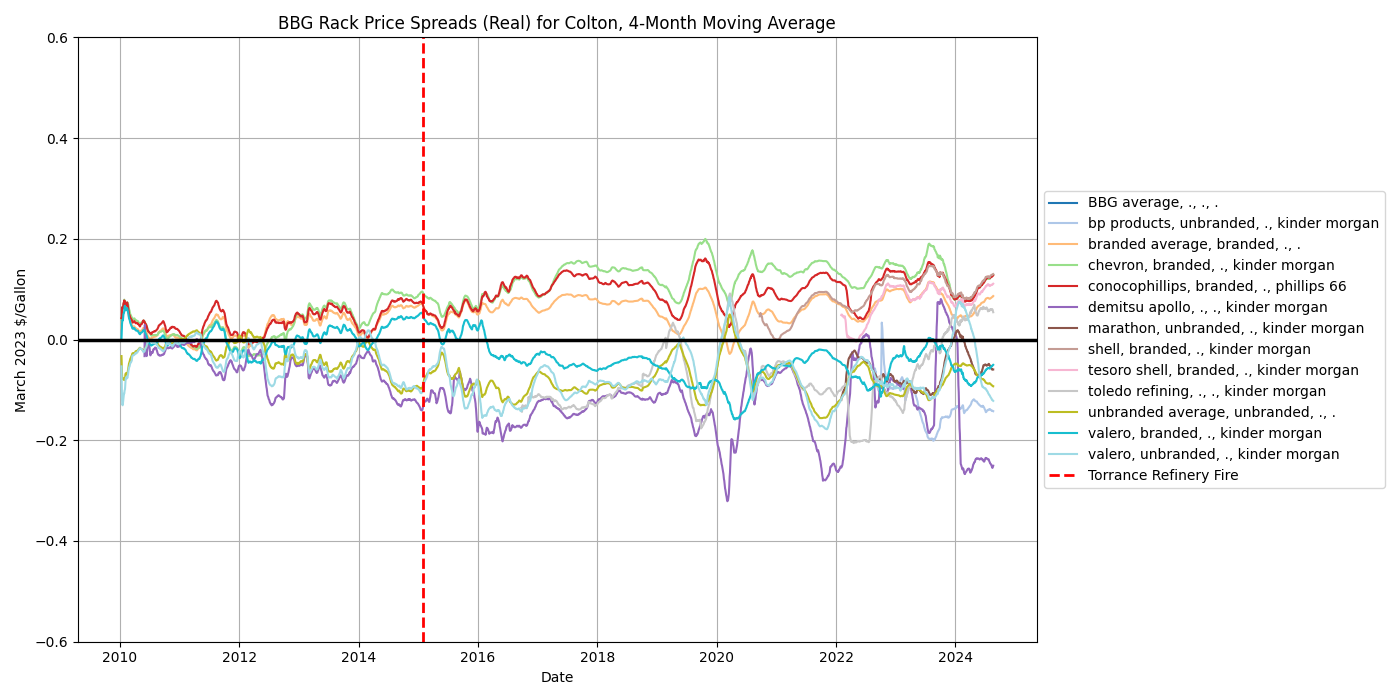
\includegraphics[width=5.5in]{colton_spread.png}\\
\raggedright Colton has the usual branded-unbranded spread. Chevron-branded, Shell-branded, ConocoPhillips-branded, and Tesoro Shell are the most elevated spreads. All are distributed by Kinder Morgan except for ConocoPhillips which is transported by itself

\subsection{Barstow} 
\centering 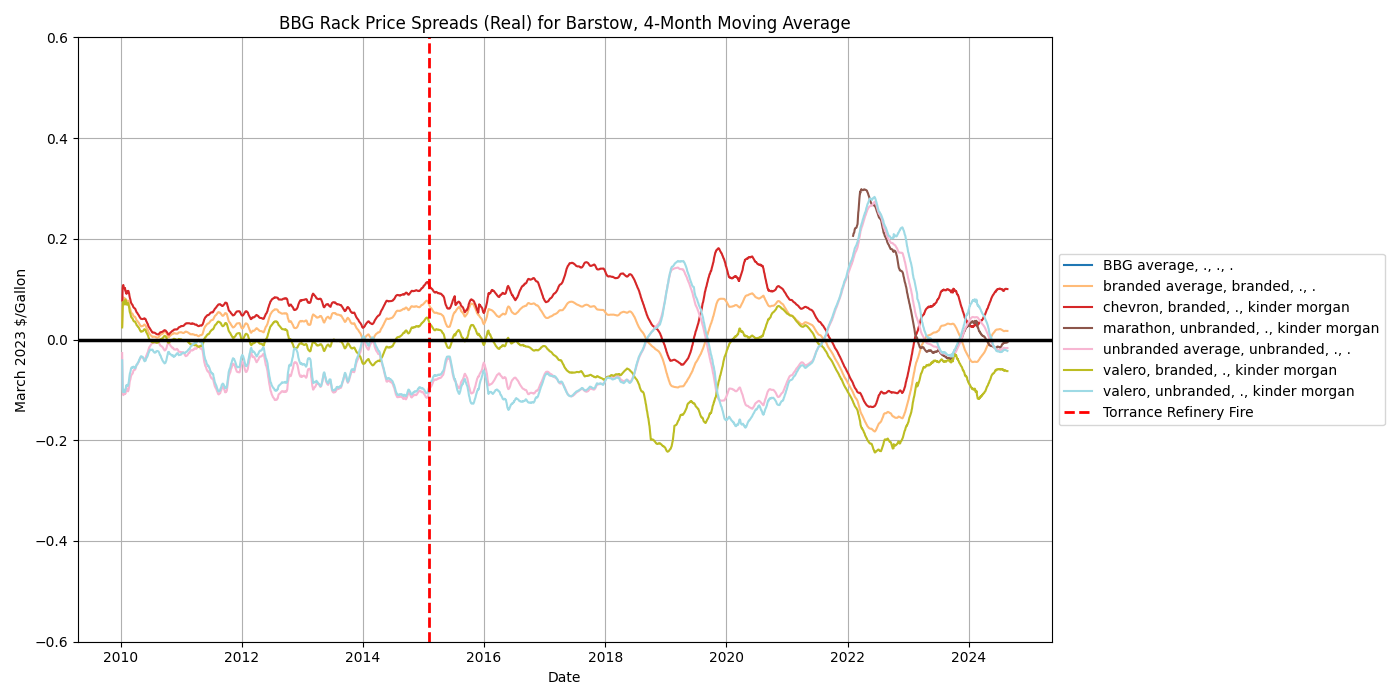
\includegraphics[width=5.5in]{barstow_spread.png}\\
\raggedright Barstow is sparse and, like Imperial, its branded-unbranded gap is inverse. This is largely due to the inversion of the Valero-unbranded and Valero-branded gasoline. All gasoline sold here is distributed by Kinder Morgan.

\subsection{Imperial}
\centering 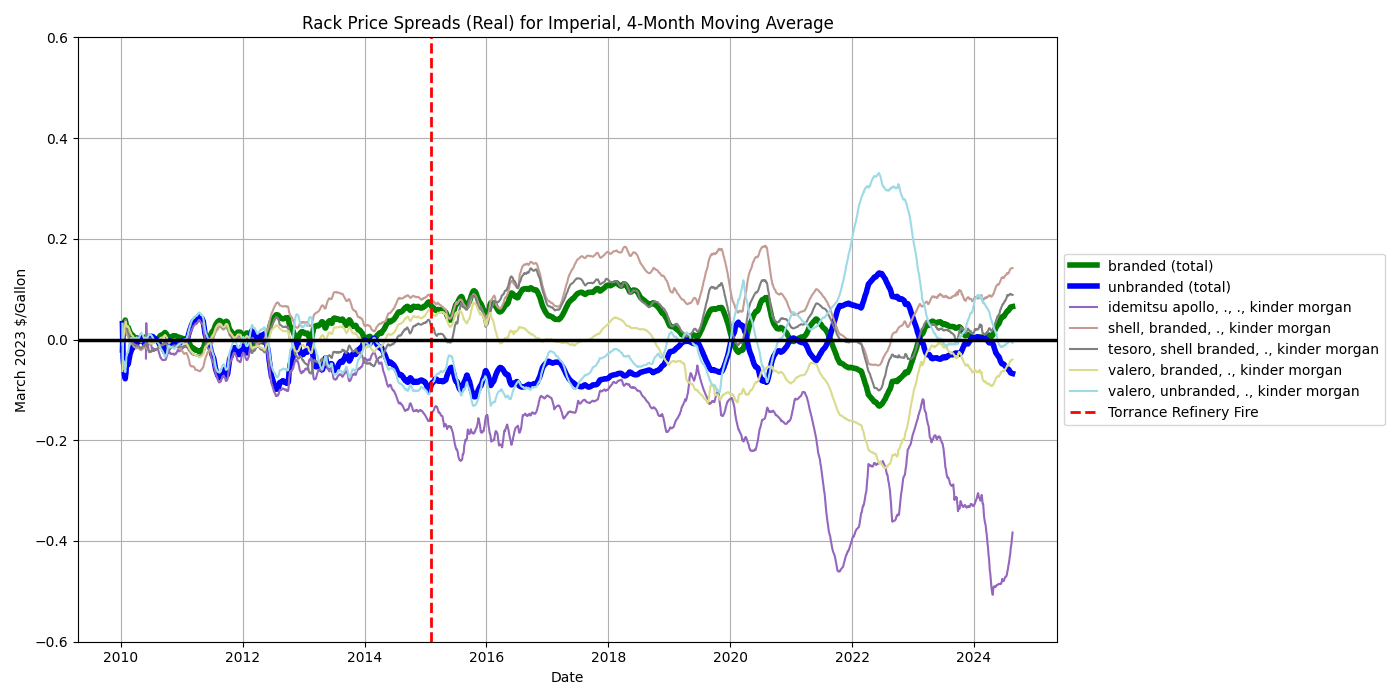
\includegraphics[width=5.5in]{imperial_spread.png}\\
\raggedright Imperial appears strange: its branded-unbranded difference is often inverted and largely follow the pattern of the Valero branded and Valero unbranded spreads, transported by Kinder Morgan which is the distributor of all gasoline sold at this location. 

\section{Comparing Across Distributors}
We can hone our analysis in multiple ways: focusing on 1) branded gasoline, 2) the most prominent refiners, and 3) the most prominent rack fuel locations. Thus, for this analysis I limit the sample to branded gasoline in Los Angeles, San Diego, San Jose, San Francisco, and Bakersfield.\footnote{I include Bakersfield because of its proximity to the only refiners outside of Los Angeles and San Francisco in all of California.} Here I sort my analysis by refiner, not city. If we follow the intuition of the argument that vertical integration lies behind the MGS, then we may expect brands that also distribute their own gasoline to have greater spreads than those that use other distributors. 

\subsection{Shell - Branded} 
\centering 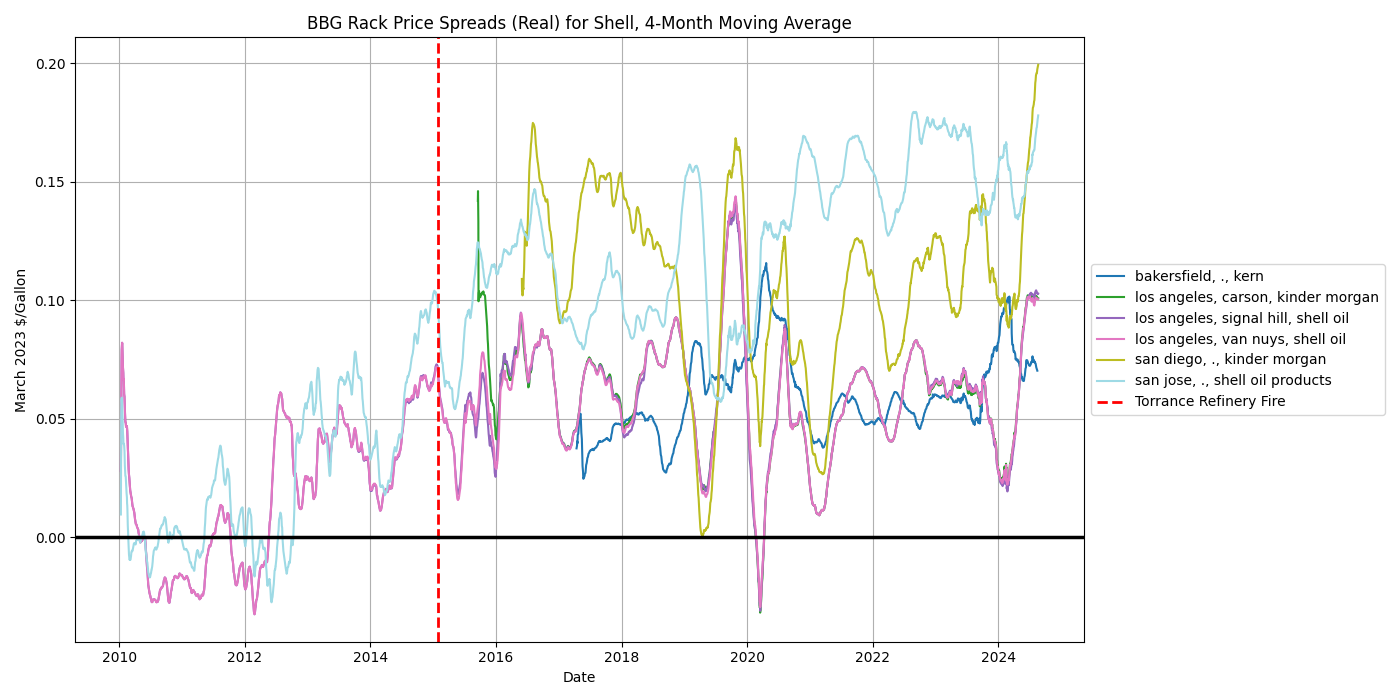
\includegraphics[width=5.5in]{shell_spread.png} \\
\raggedright As reflected above, Shell-branded gasoline's rack prices is significantly greater than the average rack price, across cities. Also of note is that for Los Angeles, the location of the Shell refinery is largely irrelevant as to the rack price. Interestingly, two of the three Los Angeles refineries are distributed by shell while the third is distributed by Kinder Morgan--and there appears to be no difference between the three. 

\subsection{Valero - Branded} 
\centering 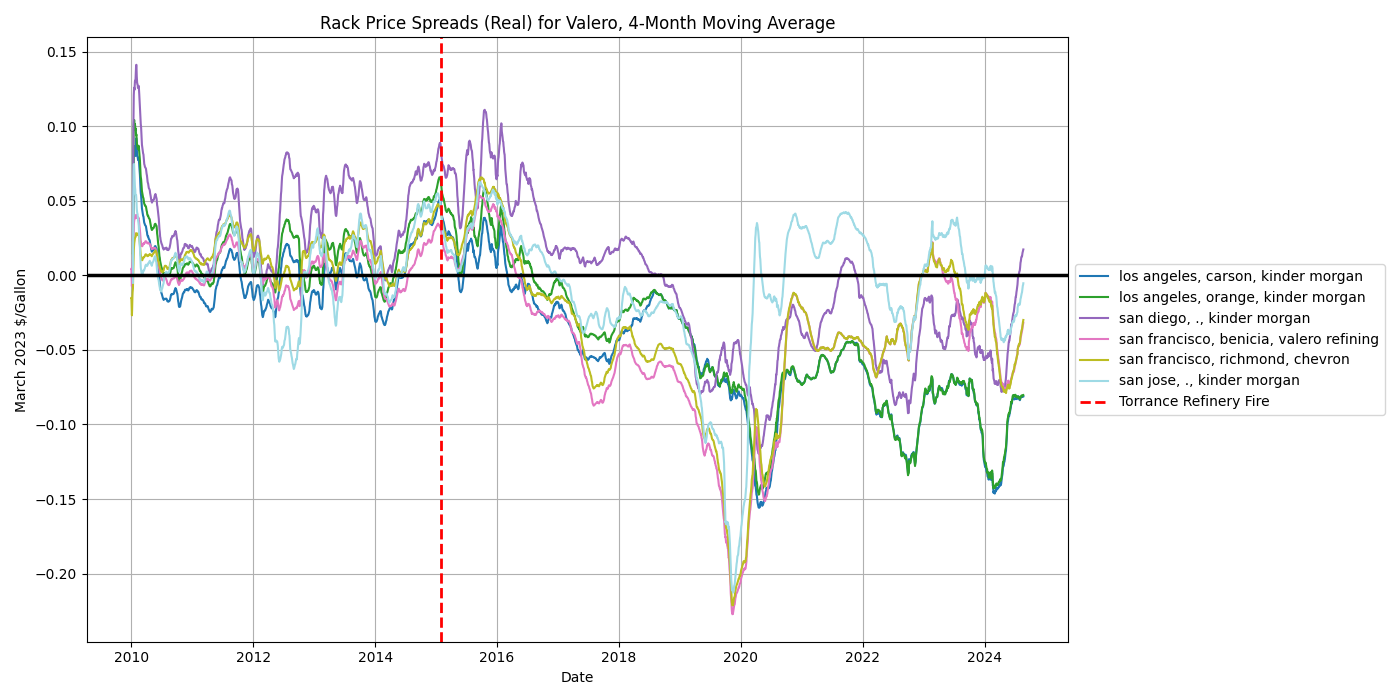
\includegraphics[width=5.5in]{valero_spread.png} \\
\raggedright Valero, even restricting to branded gasoline, largely sells at a negative spread, after hovering around a mean zero pre-Torrance Refinery Fire. Interestingly, only in San Francisco does Valero distribute their own gasoline, and in that case the spread is nearly exactly the same as the spread for the Valero refinery whose gas is distributed by Chevron. 

\subsection{Chevron - Branded} 
\centering 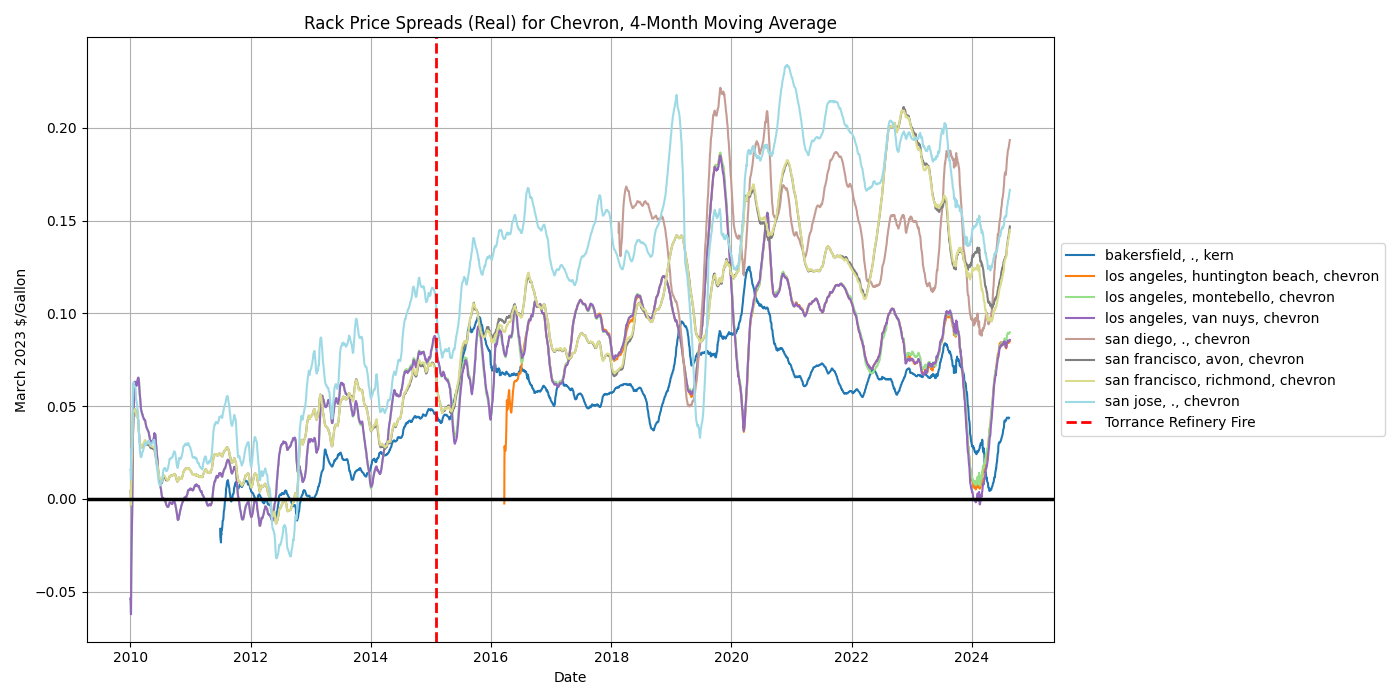
\includegraphics[width=5.5in]{chevron_spread.png} \\ 
\raggedright Chevron exhibits a similar pattern to Shell. Interestingly, every single major rack has Chevron distributing its own gasoline except for the relatively isolated Bakersfield. 

\subsection{ConocoPhillips - Branded} 
\centering 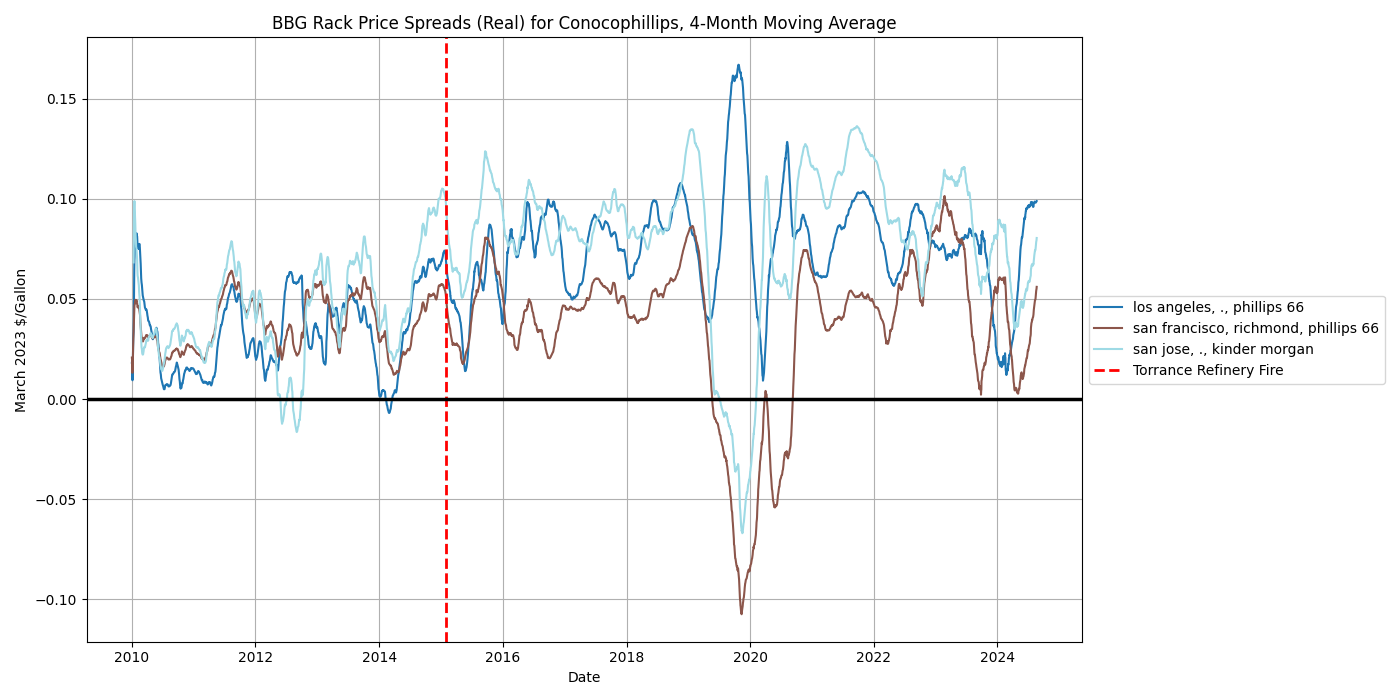
\includegraphics[width=5.5in]{conocophillips_spread.png} \\
\raggedright ConocoPhillips exhibits more volatility than the previous three major brands, with a sharp decrease in spreads in early-2019, and otherwise elevated positive spreads since approximately 2014. The San Jose, Kinder Morgan-distributed rack price is mostly the highest-elevated spread.

\end{document}